\section{Overlay Mesh}

\subsection{Self–Optimisation}
Nodes in the Mitosis network constantly try to improve their own connections. As discussed in \ref{TODO}, this should lead to a more stable system in general.

In this experiment, the positioning of peers in relation to the router is measured. Running a simulation with $n=200$ nodes for $t=1000$ ticks, the distance from each peer to the router is put in relation to the simulated network configuration of the peer. In this scenario, connection latency is configured to a random value in the range of $0.125<l<0.5$ ticks, connection establishment delay falls in the range of $0.1<1.0$ ticks and the drop probability for messages on the unreliable channel \vref{TODO} is set to $0.0<s<5.0$ percent. For simplicity, every peer is assigned values within these ranges at instantiation and those values remain static throughout the simulation.

As peers strive to acquire connections to peers with a good router link quality and a good connection quality, the hypothesis is that peers with good connection qualities will \say{bubble} towards the router. For verification, at the end of the scenario, every peer reports its network configuration parameters along with its distance to the router node. Distances are calculated in hops using the Dijkstra algorithm and treating the mesh as an undirected and unweighted graph.
\cref{fig:connection-quality-per-distance} shows the histogram of network quality settings binned by router distance. For comparability, the settings are normalised to percentages corresponding to the aforementioned ranges, with higher percentages representing the \textit{better} end of the range.

\begin{figure}[htb!]
\centering
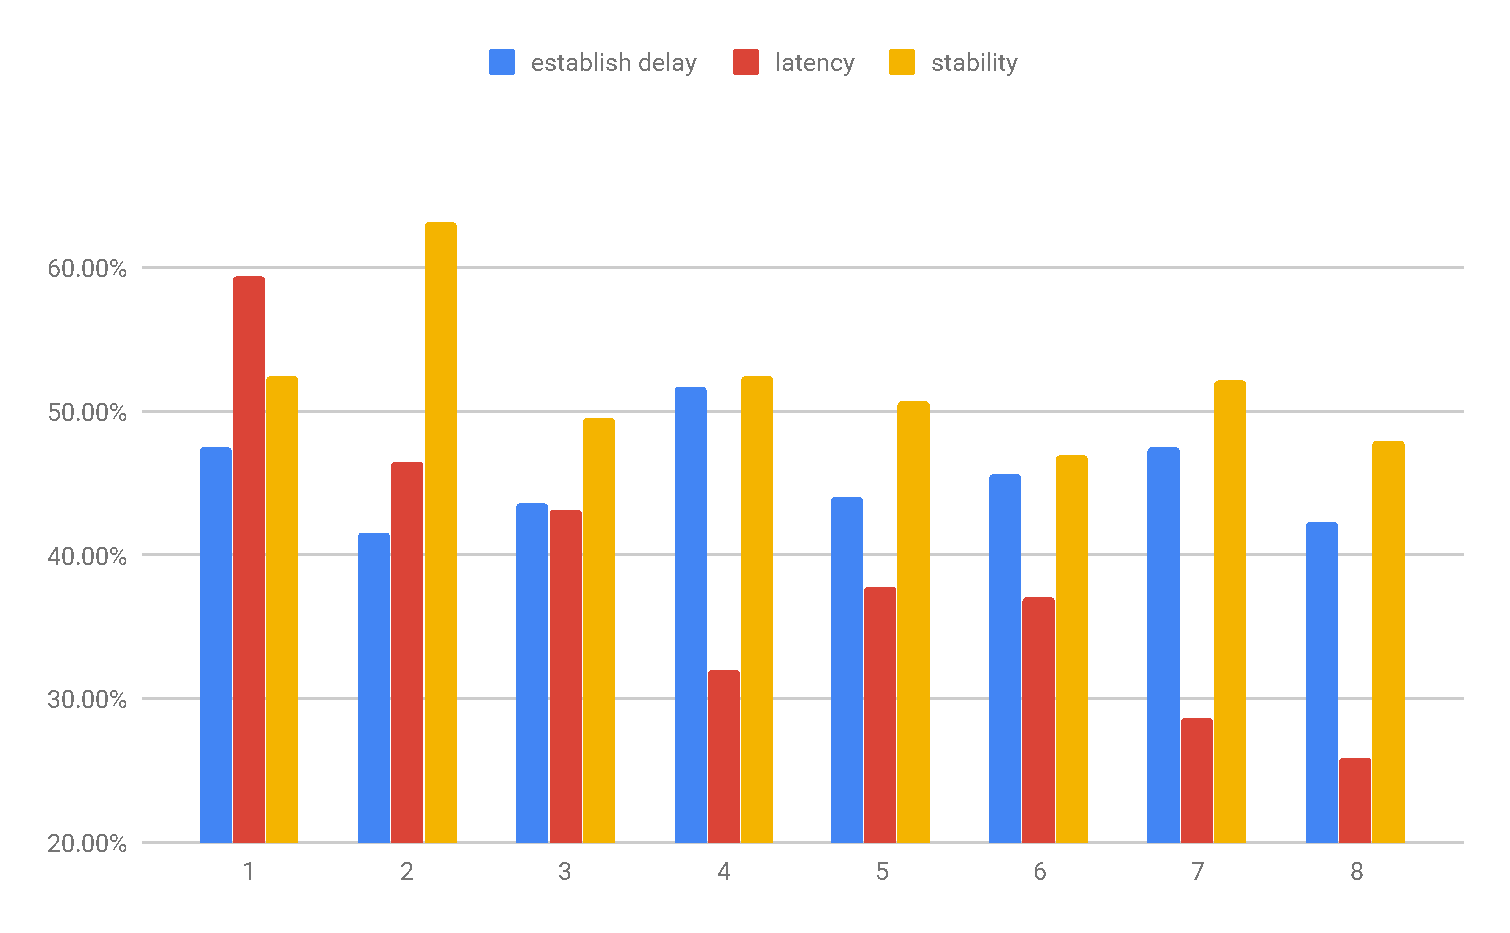
\includegraphics[width=1.0\textwidth]{graphics/analysis/connection-quality-per-distance.pdf}
\caption{Network quality of nodes in relation to their router distance}
\label{fig:connection-quality-per-distance}
\end{figure}

As to be expected, establishment delays do not show a dependency on router distance. Nodes only begin metering the quality of a connection after it has been opened. This is, in fact, a desirable behaviour, since \gls{webrtc} connections can take a while to generate \gls{ice} candidates and establish. Yet, the grade of the \gls{webrtc} connection does not relate to how long the establishment took.

The distribution of average connection latency per router distance is in line with the hypothesis. Nodes with below average latency (circa $l<0.27$) have acquired direct connections to the \router node, while nodes with only half as responsive connections have been pushed outwards to be leaf nodes.

The stability for the unreliable channel shows a distribution proximate to the latency, but not as clear. Nodes with low message drop probabilities, accumulate to distance levels one and two, yet the falloff is not as distinctive. This can be explained by looking back at the utilisation of the unreliable channel in \vref{TODO-ping-pong}: The \gls{tq} of the connection meter is intended to access the duplexity of the connection and the responsiveness of the peer. However, in the simulation, the drop probability is applied to both incoming and outgoing messages.

\subsection{Ingress Rates}

For a \gls{p2p} network to reach its potential scale, not only does it need to retain a high number of peers, it needs to take them in at a high rate. In real–world applications users can join and exit in unpredictable bursts, which can cause queues at the entry point or leaf gaps in the mesh.

The Mitosis mesh design envisions a clustered landscape \vref{todo-clusters}, where peers are associated to a router by a signal server.

\cref{fig:ingress-rates} is cool.

\begin{figure}[htb!]
\centering
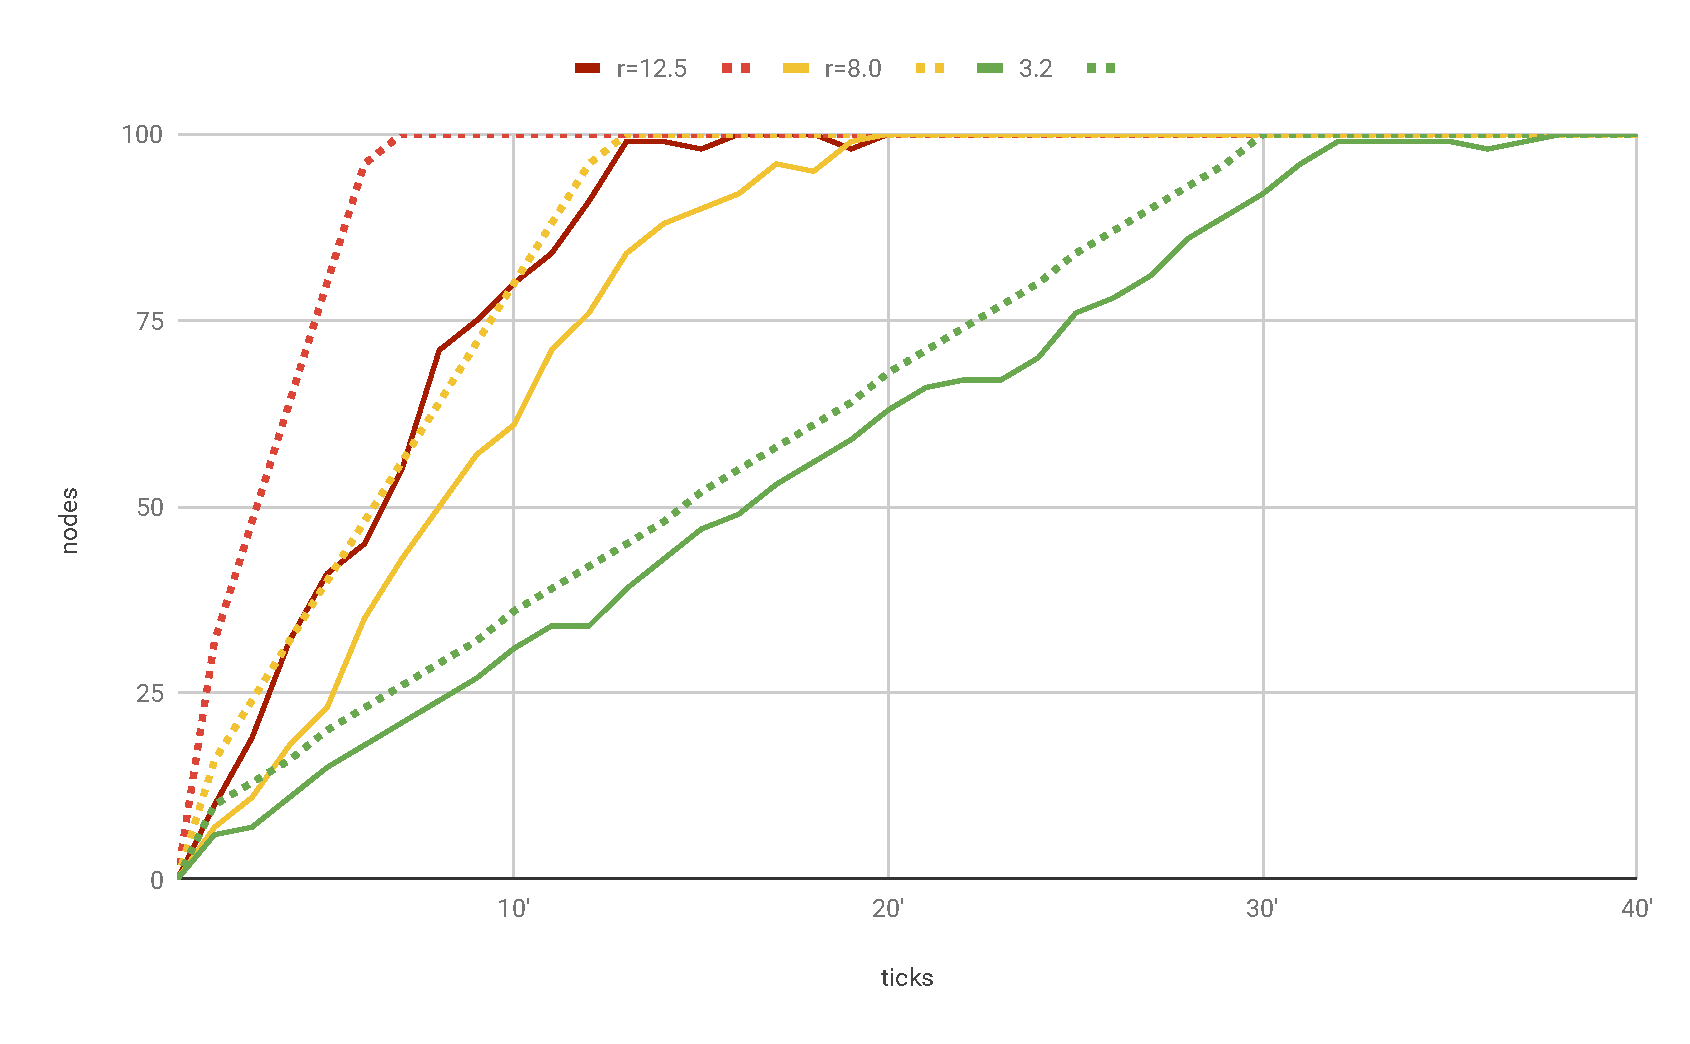
\includegraphics[width=1.0\textwidth]{graphics/analysis/ingress-final.pdf}
\caption{Ingress rates in relation to join rates in nodes per tick}
\label{fig:ingress-rates}
\end{figure}
